% Pressurized Water Reactor
% Author: Gloria Faccanoni <http://www.science.unitn.it/~gloria/home.htm>
%
\documentclass{standalone}
\usepackage{SIunits}
\usepackage[dvipsnames]{xcolor}
\usepackage{tikz}
\usetikzlibrary{decorations.pathmorphing}

% centrar bombes
% canviar turbina

\begin{document}
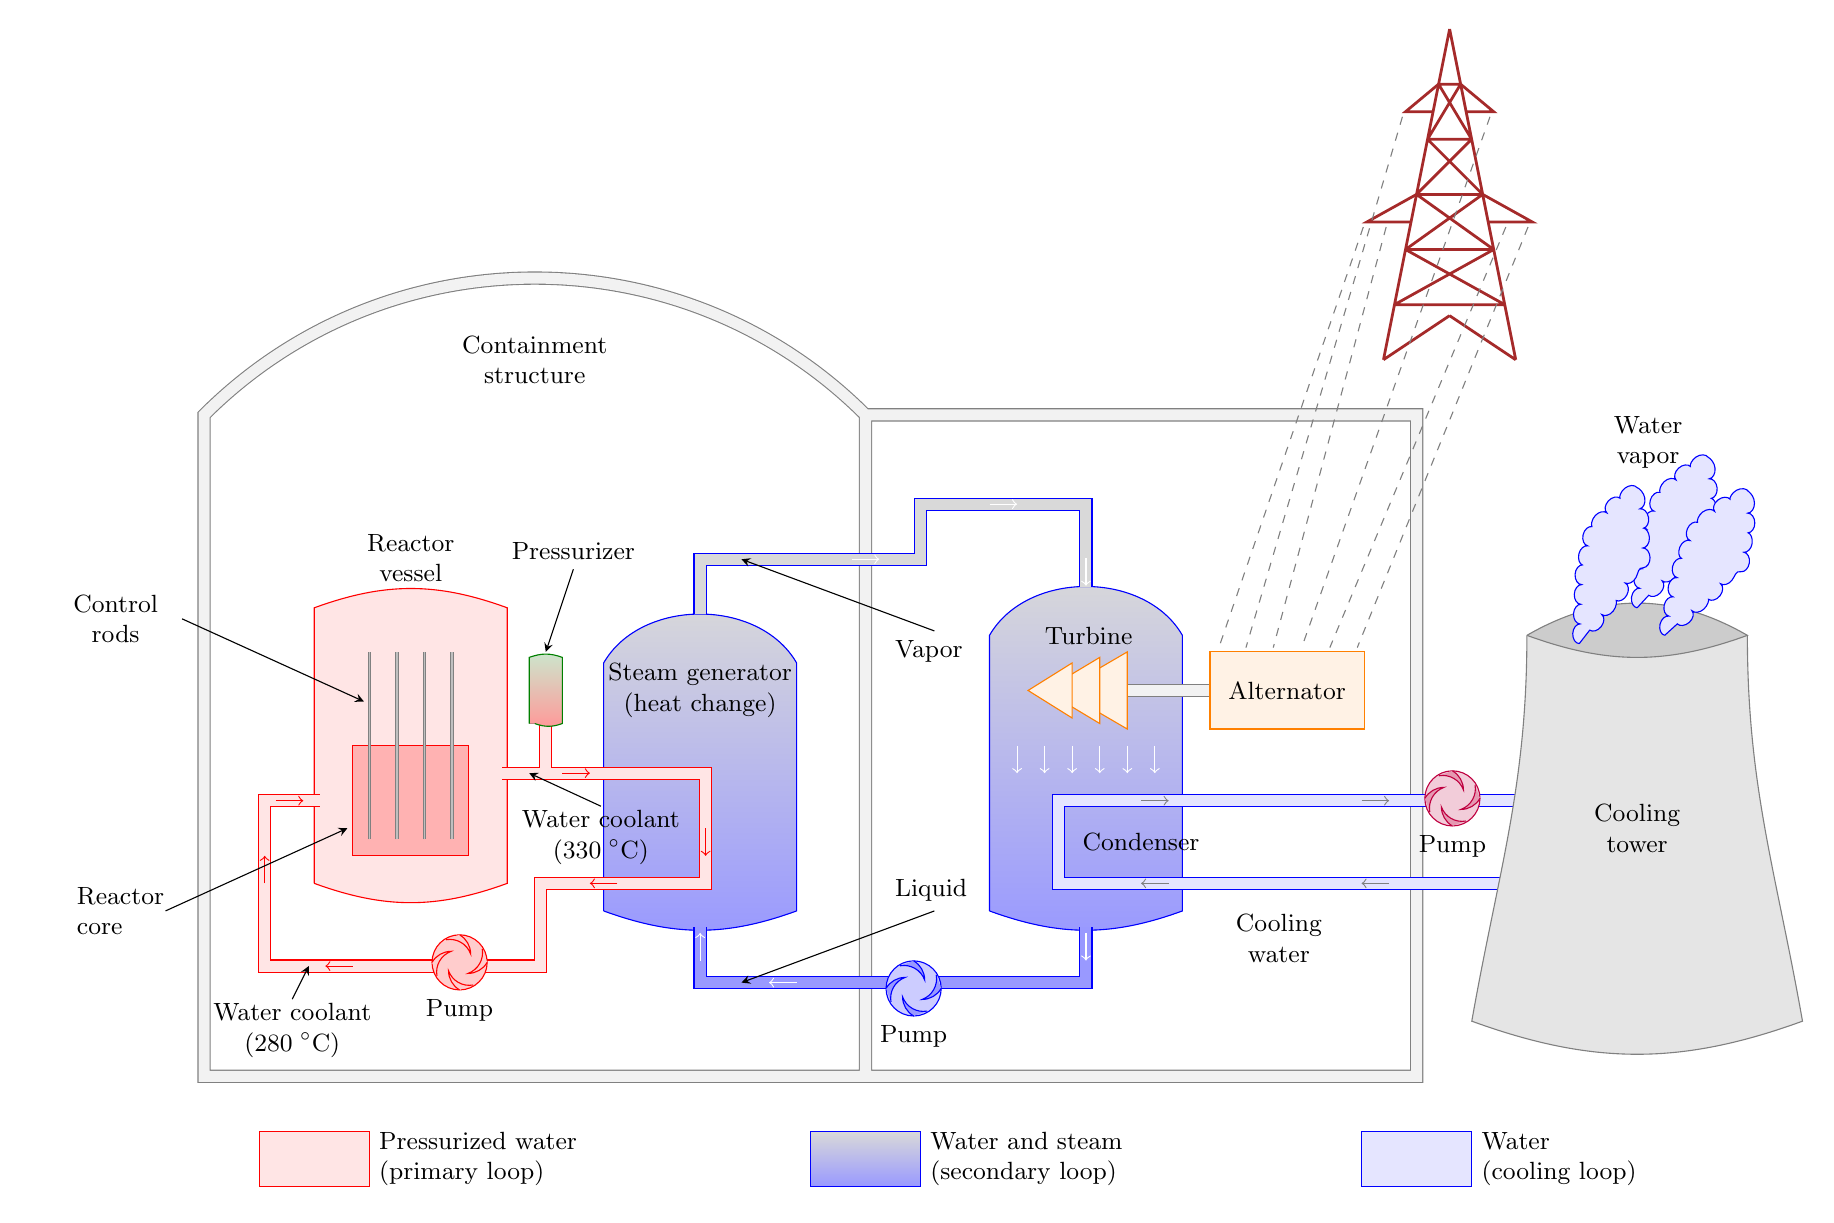
\begin{tikzpicture}[
    scale=0.7,
    annotline/.style = {stealth-},
    arrows1loop/.style={->,red},
    arrows2loop/.style={->,white},
    arrows3loop/.style={->,draw=Gray},
  ]
  \draw[draw=Gray,double=Gray!10,double distance=4pt]
  (12,12) to[out=135,in=45](0,12)--(0,0)--(22,0)--(22,12)--(12,12)--(12,0);
  \node[text width=4cm, text centered,font=\small] at (6,13)
  {Containment\\structure};
  % legend
  \begin{scope}[yshift=-2cm]
    \filldraw[draw=red,fill=red!10] (1,0) rectangle ++(2,1);
    \node[text width=4cm, font=\small,right] at (3,0.5)
    {Pressurized water\\(primary loop)};
    \filldraw[draw=blue,bottom color=blue!40,top color=Gray!30]
    (11,0) rectangle ++(2,1);
    \node[text width=4cm, font=\small,right] at (13,0.5)
    {Water and steam\\(secondary loop)};
    \filldraw[draw=Blue,fill=Blue!10] (21,0) rectangle ++(2,1);
    \node[text width=4cm, font=\small,right] at (23,0.5)
    {Water\\(cooling loop)};
  \end{scope}
  % 2nd loop --------------------------------------------------------------------
  \begin{scope}[xshift=7.25cm,yshift=3cm]
    % vessel left
    \filldraw[draw=blue,bottom color=blue!40,top color=Gray!30]
    (0,0) to[out=-20,in=200] (3.5,0) --
    (3.5,4.5) to[out=120,in=60] (0,4.5) -- (0,0);
    % vessel right
    \filldraw[draw=blue,bottom color=blue!40,top color=Gray!30,xshift=7cm]
    (0,0) to[out=-20,in=200] (3.5,0) --
    (3.5,5) to[out=120,in=60] (0,5) -- (0,0);
    % circuits
    \draw[draw=blue,double=blue!40,double distance=4pt]
    (1.75,-0.3) -- ++(0,-1) -- ++(7,0) -- ++(0,1);
    \draw[draw=blue,double=Gray!30,double distance=4pt]
    (1.75,5.38) -- ++(0,1) -- ++(4,0) -- ++(0,1) -- ++(3,0) -- ++(0,-1.5);
    % arrows
    \draw[arrows2loop] (3.5,-1.3) -- (3,-1.3);
    \draw[arrows2loop] (1.75,-0.9) -- (1.75,-0.4);
    \draw[arrows2loop] (4.5,6.38) -- (5,6.38);
    \draw[arrows2loop] (7,7.38) -- (7.5,7.38);
    \draw[arrows2loop] (8.75,6.4) -- (8.75,5.9);
    \draw[arrows2loop] (8.75,-0.4) -- (8.75,-0.9);
    %
    \foreach \x in {0.5,1,...,3}
    \draw[arrows2loop,xshift=7cm] (\x,3) -- (\x,2.5);
    % labels
    \draw[annotline] (2.5,-1.3) -- ++(3.5,1.3)
    node[text width=1cm,font=\small,above] {Liquid};
    \draw[annotline] (2.5,6.38) -- ++(3.5,-1.3)
    node[text width=1cm,font=\small,below] {Vapor};
    % pump
    \begin{scope}[xshift=160,yshift=-40]
      \filldraw[fill=Blue!20,draw=Blue] (0,0) circle (0.5cm);
      \node[below,font=\small] at (0,-0.5) {Pump};
      \filldraw[fill=Blue!40,draw=Blue,yshift=-0.5cm]
      (0,0) arc (240:180:0.4cm)  arc (200:280:0.4cm) ;
      \filldraw[fill=Blue!40,draw=Blue,yshift=+0.5cm,rotate=180]
      (0,0) arc (240:180:0.4cm)  arc (200:280:0.4cm) ;
      \filldraw[fill=Blue!40,draw=Blue,xshift=+0.5cm,rotate=90]
      (0,0) arc (240:180:0.4cm)  arc (200:280:0.4cm) ;
      \filldraw[fill=Blue!40,draw=Blue,xshift=-0.5cm,rotate=-90]
      (0,0) arc (240:180:0.4cm)  arc (200:280:0.4cm) ;
    \end{scope}
    % generator ...
    \draw[xshift=6.5cm,draw=Gray,double=Gray!10,double distance=4pt]
    (3,4) -- ++(2,0);
    \filldraw[xshift=6.5cm,fill=orange!10,draw=orange]
    (1.8,4) -- (3.0,3.3) -- (3.0,4.7) -- cycle;
    \filldraw[xshift=6.5cm,fill=orange!10,draw=orange]
    (1.5,4) -- (2.5,3.4) -- (2.5,4.6) -- cycle;
    \filldraw[xshift=6.5cm,fill=orange!10,draw=orange]
    (1.2,4) -- (2  ,3.5) -- (2  ,4.5) -- cycle;
    \filldraw[xshift=6.5cm,fill=orange!10,draw=orange]
    (4.5,3.3) rectangle (7.3,4.7);
    %labels
    \node[text width=3cm, text centered,font=\small] at (1.75,4)
    {Steam generator\\ (heat change)};
    \node[text width=2cm, text centered,font=\small] at (8.8,5) {Turbine};
    \node[text width=2cm, text centered,font=\small] at (12.4,4) {Alternator};
    % transmission lines
    \node (aa) at (11.1,4.6) {};
    \node (bb) at (11.6,4.6) {};
    \node (cc) at (12.1,4.6) {};
    \node (dd) at (12.6,4.6) {};
    \node (ee) at (13.1,4.6) {};
    \node (ff) at (13.6,4.6) {};

  \end{scope}
  % 3 loop --------------------------------------------------------------------
  \begin{scope}[xshift=23cm,yshift=1cm]
    % circuit
    \draw[draw=Blue,double=Blue!10,double distance=4pt]
    (1,2.5) -- ++(-8.5,0) -- ++(0,+1.5) -- ++(8.5,0);
    % arrows
    \draw[arrows3loop] (-5.5,2.5) -- (-6,2.5);
    \draw[arrows3loop] (-1.5,2.5) -- (-2,2.5);
    \draw[arrows3loop] (-6,4) -- (-5.5,4);
    \draw[arrows3loop] (-2,4) -- (-1.5,4);
    % tower
    \filldraw[draw=Gray,fill=Gray!20] (1,7) to[out=270,in=80]
    (0,0) to[out=-20,in=200]
    (6,0) to[out=100,in=270]
    (5,7);
    \filldraw[draw=Gray,fill=Gray!40] (1,7) to[out=30,in=150]
    (5,7) to[out=200,in=-20]
    (1,7);
    % labels
    \node[text width=3cm, text centered,font=\small] at (3,3.5)
    {Cooling\\tower};
    \node[text width=2cm, text centered,font=\small] at (-3.5,1.5)
    {Cooling\\water};
    \node[text width=2cm, text centered,font=\small] at (-6,3.25)
    {Condenser};
    % pump
    \begin{scope}[xshift=-10,yshift=115]
      \filldraw[fill=purple!20,draw=purple] (0,0) circle (0.5cm);
      \node[below,font=\small] at (0,-0.5) {Pump};
      \filldraw[fill=purple!40,draw=purple,yshift=-0.5cm]
      (0,0) arc (240:180:0.4cm)  arc (200:280:0.4cm) ;
      \filldraw[fill=purple!40,draw=purple,yshift=+0.5cm,rotate=180]
      (0,0) arc (240:180:0.4cm)  arc (200:280:0.4cm) ;
      \filldraw[fill=purple!40,draw=purple,xshift=+0.5cm,rotate=90]
      (0,0) arc (240:180:0.4cm)  arc (200:280:0.4cm) ;
      \filldraw[fill=purple!40,draw=purple,xshift=-0.5cm,rotate=-90]
      (0,0) arc (240:180:0.4cm)  arc (200:280:0.4cm) ;
    \end{scope}
  \end{scope}
  %1 loop --------------------------------------------------------------------
  \begin{scope}[xshift=2cm,yshift=4cm]
    % Reactor vessel
    \filldraw[draw=red,fill=red!10] (0,-0.5) to[out=-20,in=200]
    (3.5,-0.5) --
    (3.5,4.5) to[out=160,in=20]
    (0,4.5) --
    (0,-0.5);
    % circuit
    \draw[draw=red,double=red!10,double distance=4pt]
    (0.1,1) --  ++(-1,0) -- ++(0,-3) -- ++(5,0) -- ++(0,1.5) --
    ++(3,0) -- ++(0,2) -- ++(-3.7,0);
    % Pressurizer
    \draw[draw=red,double=red!10,double distance=4pt] (4.2,1.6) -- ++(0,0.8);
    \filldraw[draw=Green,bottom color=red!40,top color=Green!20]
    (4,2.4) to[out=-20,in=200]
    (4.5,2.4) --
    (4.5,3.6) to[out=160,in=20]
    (3.9,3.6) --
    (3.9,2.4);
    % arrows
    \draw[arrows1loop] (-0.7,1) -- (-0.2,1);
    \draw[arrows1loop] (-0.9,-0.5) -- (-0.9,0);
    \draw[arrows1loop] (0.7,-2) -- (0.2,-2);
    \draw[arrows1loop] (4.5,1.5) -- (5,1.5);
    \draw[arrows1loop] (7.1,0.5) -- (7.1,0);
    \draw[arrows1loop] (5.5,-0.5) -- (5,-0.5);

    % pump
    \begin{scope}[xshift=75,yshift=-55,fill=red!20,draw=red]
      \filldraw (0,0) circle (0.5cm);
      \node[below,font=\small] at (0,-0.5) {Pump};
      \filldraw[yshift=-0.5cm] (0,0) arc (240:180:0.4cm)  arc (200:280:0.4cm) ;
      \filldraw[yshift=+0.5cm,rotate=180]
      (0,0) arc (240:180:0.4cm)  arc (200:280:0.4cm) ;
      \filldraw[xshift=+0.5cm,rotate=90]
      (0,0) arc (240:180:0.4cm)  arc (200:280:0.4cm) ;
      \filldraw[xshift=-0.5cm,rotate=-90]
      (0,0) arc (240:180:0.4cm)  arc (200:280:0.4cm) ;
    \end{scope}
    % reactor core
    \filldraw[fill=red!30,draw=red] (0.7,0) rectangle (2.8,2);

    % control rods
    \foreach \x in {1.0,1.5,2.0,2.5}
    \draw[draw=Gray,double=Gray!50,double distance=0.5pt] (\x,0.3) -- (\x,3.7);

    %labels
    \draw[annotline] (0.6,0.5) -- ++(-3.3,-1.5)
    node[text width=1cm,font=\small,left] {Reactor core};
    \node[text width=2cm, text centered,font=\small] at (1.75,5.4) {Reactor vessel};
    \draw[annotline] (0.9,2.8) -- ++(-3.3,1.5)
    node[text width=2cm, text centered,font=\small,left=-8pt] {Control\\rods};
    \draw[annotline] (4.2,3.7) -- ++(0.5,1.5)
    node[text width=2cm, text centered,font=\small,above] {Pressurizer};
    \draw[annotline] (3.9,1.5) -- ++(1.3,-0.6)
    node[text width=2.4cm, text centered,below=-2pt,font=\small]
    {Water coolant (\unit{330}{\degreecelsius})};
    \draw[annotline] (-0.1,-2) -- ++(-0.3,-0.6)
    node[text width=2.4cm, text centered,below=-2pt,font=\small]
    {Water coolant (\unit{280}{\degreecelsius})};
  \end{scope}
  % clouds ----------------------------------
  \begin{scope}[xshift=26cm,yshift=10cm, fill=blue!10, draw=Blue,
      decoration={bumps,segment length=0.5cm}]
    \filldraw[yshift=-1.5cm,rotate=-25,decorate]
    (0,0) -- ++(-0.4,1.25)-- ++(-0.1,0.75)-- ++(0.2,0.5)-- ++(0.3,0.5)--
    ++(0.3,-0.5)-- ++(0.2,-0.5)-- ++(-0.1,-0.75)-- ++(-0.4,-1.25);
    \filldraw[xshift=0.5cm,yshift=-2cm,rotate=-30,decorate]
    (0,0) -- ++(-0.4,1.25)-- ++(-0.1,0.75)-- ++(0.2,0.5)-- ++(0.3,0.5)--
    ++(0.3,-0.5)-- ++(0.2,-0.5)-- ++(-0.1,-0.75)-- ++(-0.4,-1.25);
    \filldraw[xshift=-1.05cm,yshift=-2.15cm,rotate=-20,decorate]
    (0,0) -- ++(-0.4,1.25)-- ++(-0.1,0.75)-- ++(0.2,0.5)-- ++(0.3,0.5)--
    ++(0.3,-0.5)-- ++(0.2,-0.5)-- ++(-0.1,-0.75)-- ++(-0.4,-1.25);
    %labels
    \node[text width=1cm, text centered,font=\small] at (0.2,1.5) {Water vapor};
  \end{scope}

  % palo della luce
  \begin{scope}[xscale=0.2,xshift=113cm,yshift=19cm,line width=1pt,Brown]
    \draw (0,0) -- (-6,-6)
    (0,0) -- ( 6,-6)
    (-1,-1) -- ( 1,-1)
    (-1,-1) -- ( 2,-2)
    ( 1,-1) -- (-2,-2)
    (-2,-2) -- ( 2,-2)
    (-2,-2) -- ( 3,-3)
    ( 2,-2) -- (-3,-3)
    ( 3,-3) -- (-3,-3)
    (-3,-3) -- ( 4,-4)
    ( 3,-3) -- (-4,-4)
    ( 4,-4) -- (-4,-4)
    (-4,-4) -- ( 5,-5)
    ( 4,-4) -- (-5,-5)
    ( 5,-5) -- (-5,-5)
    (-6,-6) -- ( 0,-5.2)
    ( 6,-6) -- ( 0,-5.2);
    \draw (-1.5,-1.5) -- (-4,-1.5) -- (-1,-1)
    ( 1.5,-1.5) -- ( 4,-1.5) -- ( 1,-1);
    \path (-4,-1.4) node (a) {}
    ( 4,-1.4) node (b) {};
    \draw[line width=1pt,Brown] (-3.5,-3.5) -- (-7.5,-3.5) -- (-3,-3)
    ( 3.5,-3.5) -- ( 7.5,-3.5) -- ( 3,-3);
    \path (-7.5,-3.4) node (c) {}
    ( 7.5,-3.4) node (d) {}
    (-5.5,-3.4) node (e) {}
    ( 5.5,-3.4) node (f) {};
  \end{scope}
  % transmission lines
  \draw[dashed,Gray] (c) -- (aa)
  (a) -- (bb)
  (e) -- (cc)
  (b) -- (dd)
  (f) -- (ee)
  (d) -- (ff);
\end{tikzpicture}
\end{document}
